[some introductory text to the chapter]
[måste fixa tempus här]

\section{Performance of Forecasting Models}
The performance of the five decision tree-based ensemble models is assessed via MAPE, RMSE, and MAE metrics. \autoref{tab:performance} shows the scores for each model, separated by internal features and total features. Scores under the internal feature category represent the models' performance when only trained using the historical electricity consumption, while total features refers to the combination of internal and external features. The best performing model is XGBoost, with 14.96\% errors on the total feature set. RF shows the worst performance with 16.33\% errors and considerably higher RMSE and MAE scores on the total feature set, compared to the other models.

Results indicate that the inclusion of external factors does help with improving the forecast accuracy in terms of MAPE, but that MAE and especially RMSE scores may actually worsen, a pattern that is apparent among all models. MAPE is more sensitive to errors on small consumption values, while RMSE is more sensitive to high consumption values and outliers. This suggests that the external factors help with increasing forecast accuracy for households with a lower and more stable consumption, while households with a high or varied consumption do not benefit from the external factors.

\begin{table}[H]
    \centering
    \caption{Performance of forecasting models.}
    \label{tab:performance}
    \small
    \begin{tabularx}{\linewidth}{l *{6}{R}}
                       & \multicolumn{3}{c}{\textbf{Internal features}} & \multicolumn{3}{c}{\textbf{Total features}}                                                                                      \\
        \cmidrule(lr){2-4} \cmidrule(lr){5-7}
        \textbf{Model} & \textbf{MAPE (\%)}                             & \textbf{RMSE (kWh)}                         & \textbf{MAE (kWh)} & \textbf{MAPE (\%)} & \textbf{RMSE (kWh)} & \textbf{MAE (kWh)} \\
        \midrule
        RF             & 16.34                                          & 142.47                                      & 65.93              & 16.33              & 171.47              & 74.68              \\
        GBM            & 15.67                                          & 144.07                                      & 64.49              & 15.07              & 154.97              & 66.67              \\
        XGBoost        & 15.40                                          & 144.12                                      & 63.94              & 14.96              & 153.55              & 65.46              \\
        LightGBM       & 15.67                                          & 150.21                                      & 66.09              & 15.18              & 159.54              & 67.03              \\
        CatBoost       & 15.73                                          & 152.85                                      & 65.74              & 16.05              & 150.07              & 66.52              \\
        %\midrule
        %Linear regression &                                                &                                             &                    & 18.47              & 161.43              & 71.98              \\
    \end{tabularx}
\end{table}

A pattern occurring for all models is that on average, the models overestimate the electricity consumption during the winter months in the beginning of the year, as illustrated in \autoref{fig:avg-actual-vs-predicted}. During the summer, the average predictions lie closer to the actual average consumption of the households. The scatter plots in \autoref{fig:scatter-plots} show that the overestimation of electricity consumption is a general trend for all models except XGBoost, indicated by the regression lines with larger slopes than the perfect prediction line. For those models, it is clear that predictions in the several thousand kWh range are commonly overestimated, while the errors for lower kWh predictions are more evenly distributed around the perfect prediction line. %This again points towards the effect of outliers on the performance of the models.

\begin{figure}[H]
    \centering
    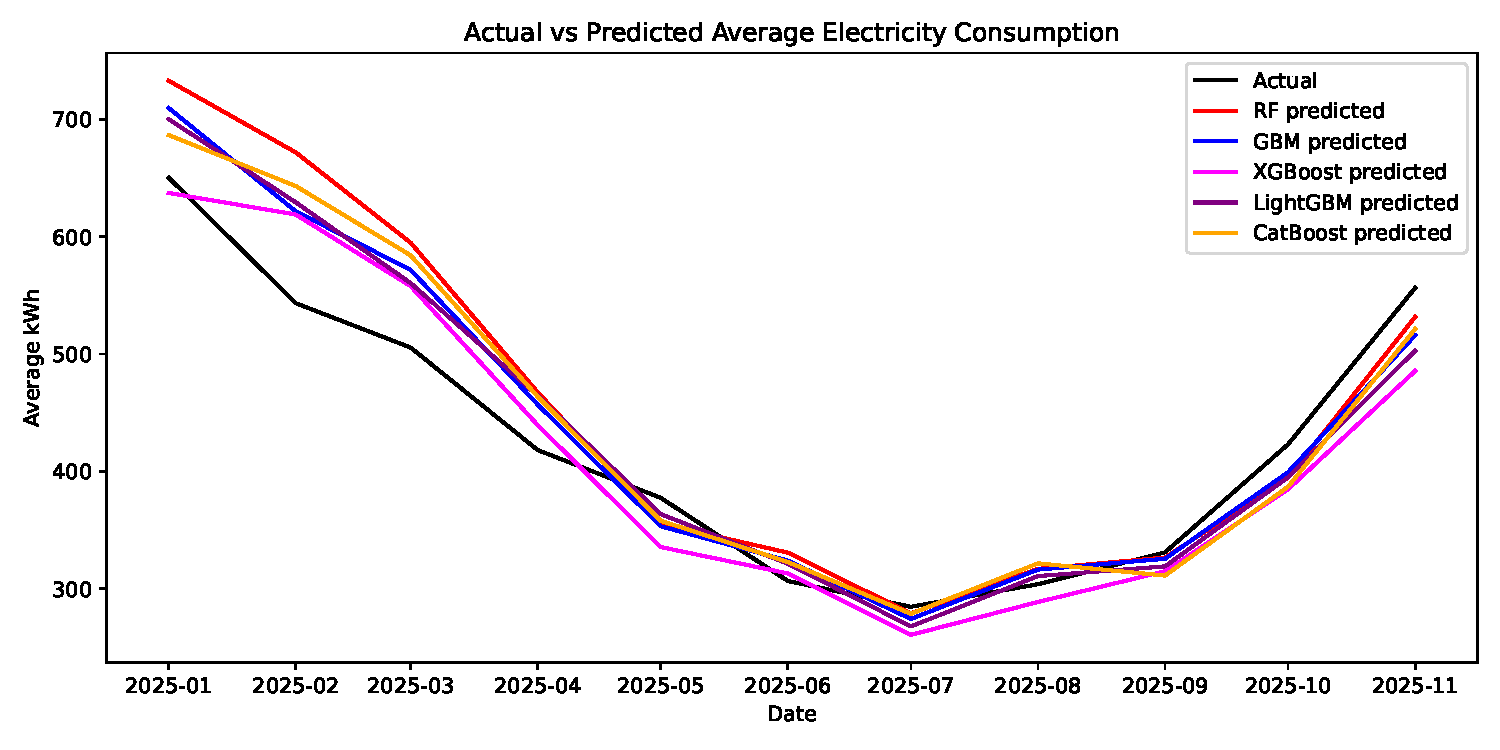
\includegraphics[width=1\linewidth]{figures/avg_predicted_vs_actual_consumption.pdf}
    \caption{Average actual versus predicted electricity consumption for all models.}
    \label{fig:avg-actual-vs-predicted}
\end{figure}

\begin{figure}[H]
    \centering
    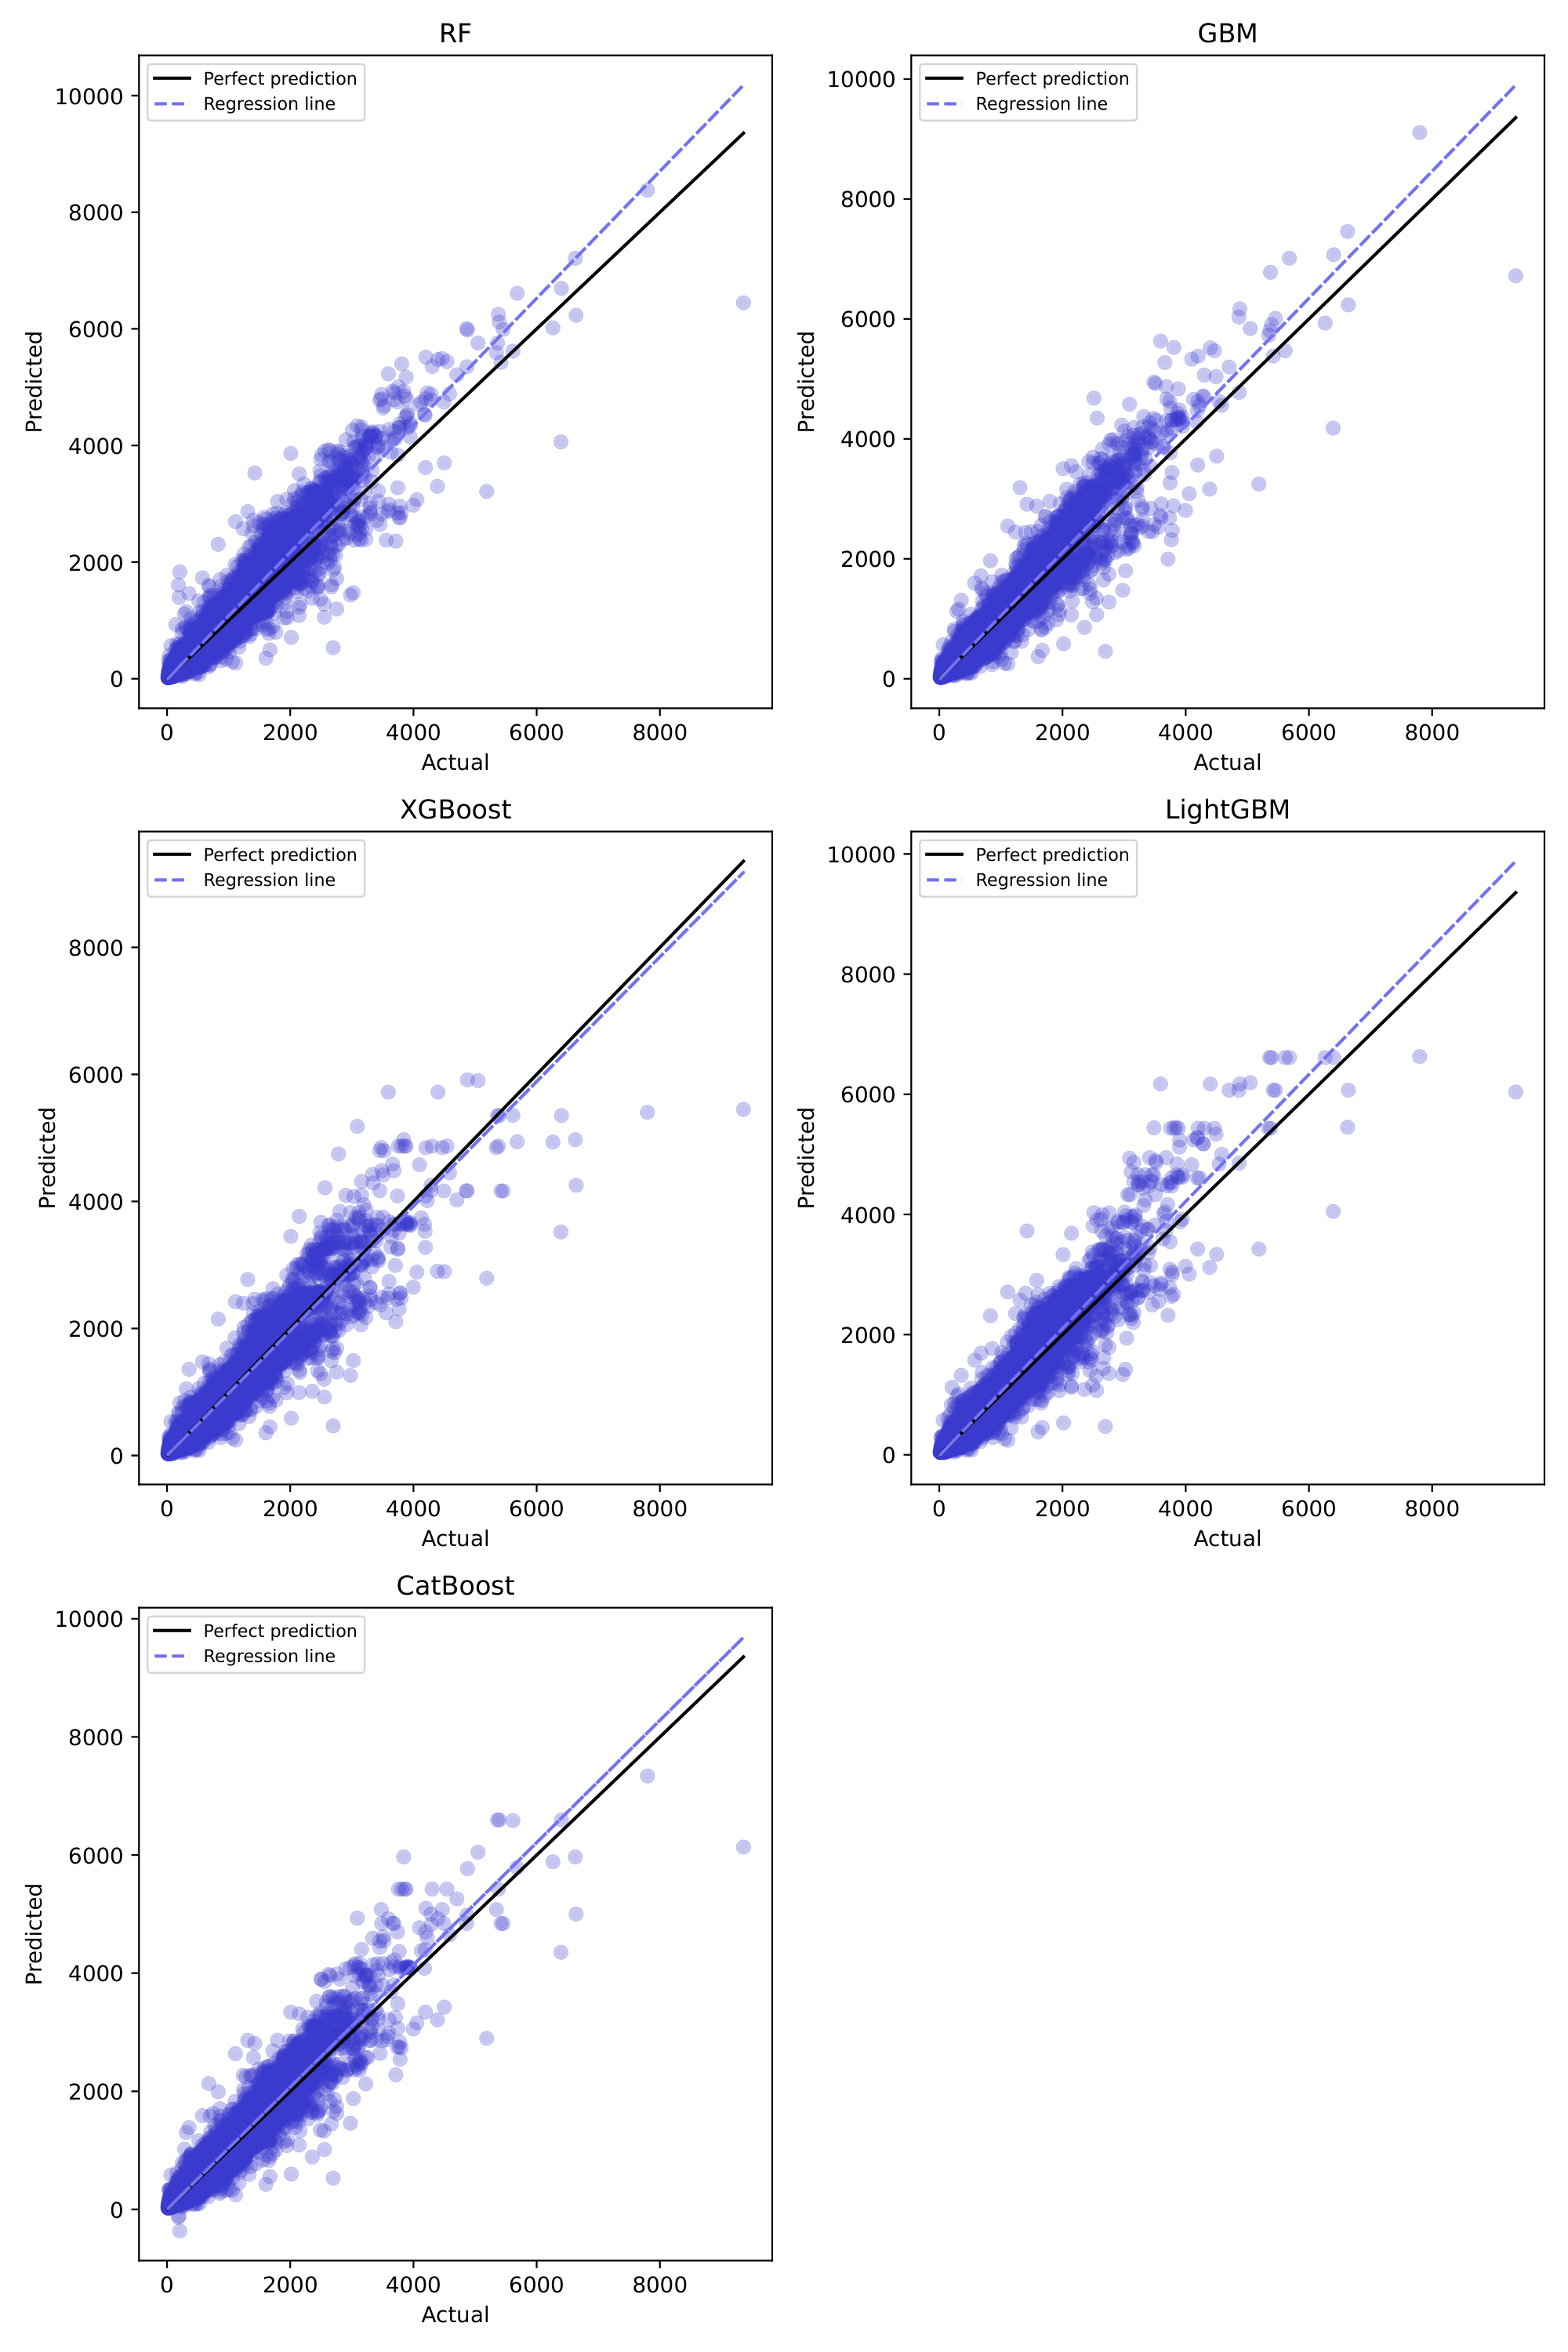
\includegraphics[width=1\linewidth]{figures/scatter_plots.png}
    \caption{Scatter plots showing prediction error distribution for each model.}
    \label{fig:scatter-plots}
\end{figure}

\subsection{Comparison with Baseline Model}

The baseline linear regression model used for comparison uses historical consumption and temperature as input variables. The past 24 months of electricity consumption and monthly average temperature was used to predict the following month's consumption. Evaluation of the linear regression model was performed using the same 2000 household sample as for the ensemble models, and the results are found in \autoref{tab:comparison-performance}. The linear regression model performs worse than the best ensemble models by roughly 3.5\% in percentage errors. RMSE and MAE scores are also worse for the linear model, especially when compared to ensemble models using only internal features.

\begin{table}[H]%[ht]
    \centering
    \caption{Performance of best ensemble model versus linear regression.}
    \label{tab:comparison-performance}
    \small
    \begin{tabularx}{\linewidth}{l r r r}
        \textbf{Model}          & \textbf{MAPE (\%)} & \textbf{RMSE (kWh)} & \textbf{MAE (kWh)} \\
        \midrule
        Best ensemble (XGBoost) & 14.96              & 153.55              & 65.46              \\
        Linear regression       & 18.47              & 161.43              & 71.98              \\
    \end{tabularx}
\end{table}

\autoref{fig:avg-actual-vs-predicted-lr} shows the average predicted monthly electricity consumption for linear regression and all ensemble models. The linear regression model shows the same tendency to overestimate the consumption during the beginning of the year as the ensemble models, while also showing a pattern of underestimating the consumption during the summer.

\begin{figure}[H]
    \centering
    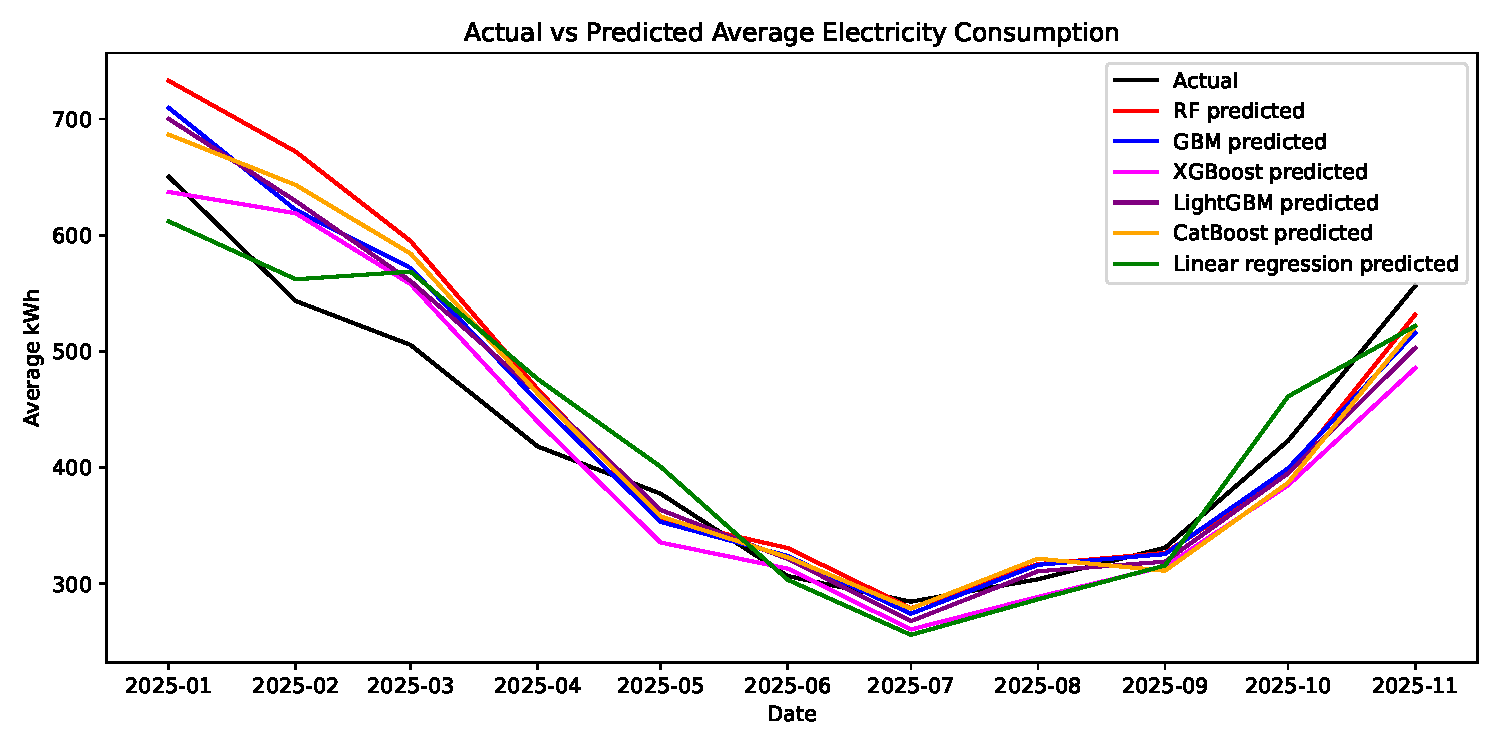
\includegraphics[width=1\linewidth]{figures/avg_predicted_vs_actual_consumption_lr.pdf}
    \caption{Average actual versus predicted electricity consumption for ensemble models and linear regression.}
    \label{fig:avg-actual-vs-predicted-lr}
\end{figure}

[maybe try LSTM and ANN for comparison too]

\section{Explainable AI Analysis of Forecasts}

All five ensemble learning models were analyzed via the SHAP method. Firstly, the models were trained using their optimal hyperparameters, and feature importance metrics were retrieved for the trained models. Secondly, a tree SHAP analysis was performed to calculate the Shapley values for all features. For the RF model, approximate SHAP values were used due to the full calculation being time-consuming for this particular model. \cref{fig:fi-shap-rf,fig:fi-shap-gbm,fig:fi-shap-xgboost,fig:fi-shap-lgbm,fig:fi-shap-catboost} show the resulting feature importance plots (left) and SHAP summary plots (right) [change to a) and b)] for each model.

Both the feature importance and SHAP analysis show that the $lag\_1$ and $lag\_12$ historical consumption features are highly influential for all models. According to the feature importance plot for GBM in \autoref{fig:fi-shap-gbm}, the model almost exclusively relies on the $lag\_1$ and $lag\_12$ features. The SHAP summary plots for all models, showing the effect of individual feature values on the prediction, also demonstrate that these features have a clear relationship where low feature values contribute to a lower predicted value, and high feature values contribute to higher predictions. Most models prioritize the $lag\_1$ feature over $lag\_12$ in their decision-making, except for RF. The $rolling\_mean\_3$ feature is ranked relatively high for all models, but the SHAP summary plots show that the feature may have a more complex relationship to the model output in some models. For GBM, XGBoost, and LightGBM, high values of the $rolling\_mean\_3$ feature contribute both to decreasing and increasing predicted values. The XGBoost model deviates from the other models by ranking the $WCT$ feature the highest in feature importance. However, the more detailed SHAP summary plot ranks the $lag\_1$ and $lag\_12$ as most influential, displaying them with a similar pattern to the other model. The SHAP summary also has a significantly lower ranking of the $WCT$ feature.

Household information features specifying residence type, and heating system were influential for the RF model, but remaining models were not as impacted by these features. The contract type feature was ranked low for all models. Even though these features commonly saw low rankings, the SHAP summaries indicate patterns where the features values had consistent impact on the SHAP values. Because of the special categorical feature handling of the CatBoost model, the SHAP summary in \autoref{fig:fi-shap-catboost} is unable to display the high/low feature value indications for these features, but it is evident that some instances of the $contract\_type$ feature had a large impact on the resulting SHAP value. In addition to the household information features, clustering of the households was performed based on their electricity consumption. The three resulting consumption groups were encoded by the $cluster$ feature. This feature was found in the lower ranks for all models.

Among the external variables, wind direction and sunshine amount are consistently ranked highly for all models. One commonly low ranked feature is the lowest cloud base feature, while remaining weather variables had a more varied impact depending on the model. The calculated weather indices $THI$ and $WCT$ also had a varied impact on the models. This can partly be attributed to the fact that the features are fully correlated with each other and with some of the weather variables [discussion probably]. The two calendar information features, $number\_of\_holidays$ and $number\_of\_days$, are commonly ranked among the less important features for the models, along with the $year$ timestamp variable. The $month$ variable, indicating the month of the year, is however ranked highly for several models.

\begin{figure}[H]
    \centering
    \makebox[\linewidth][c]{%
        \hspace{-1.5cm}
        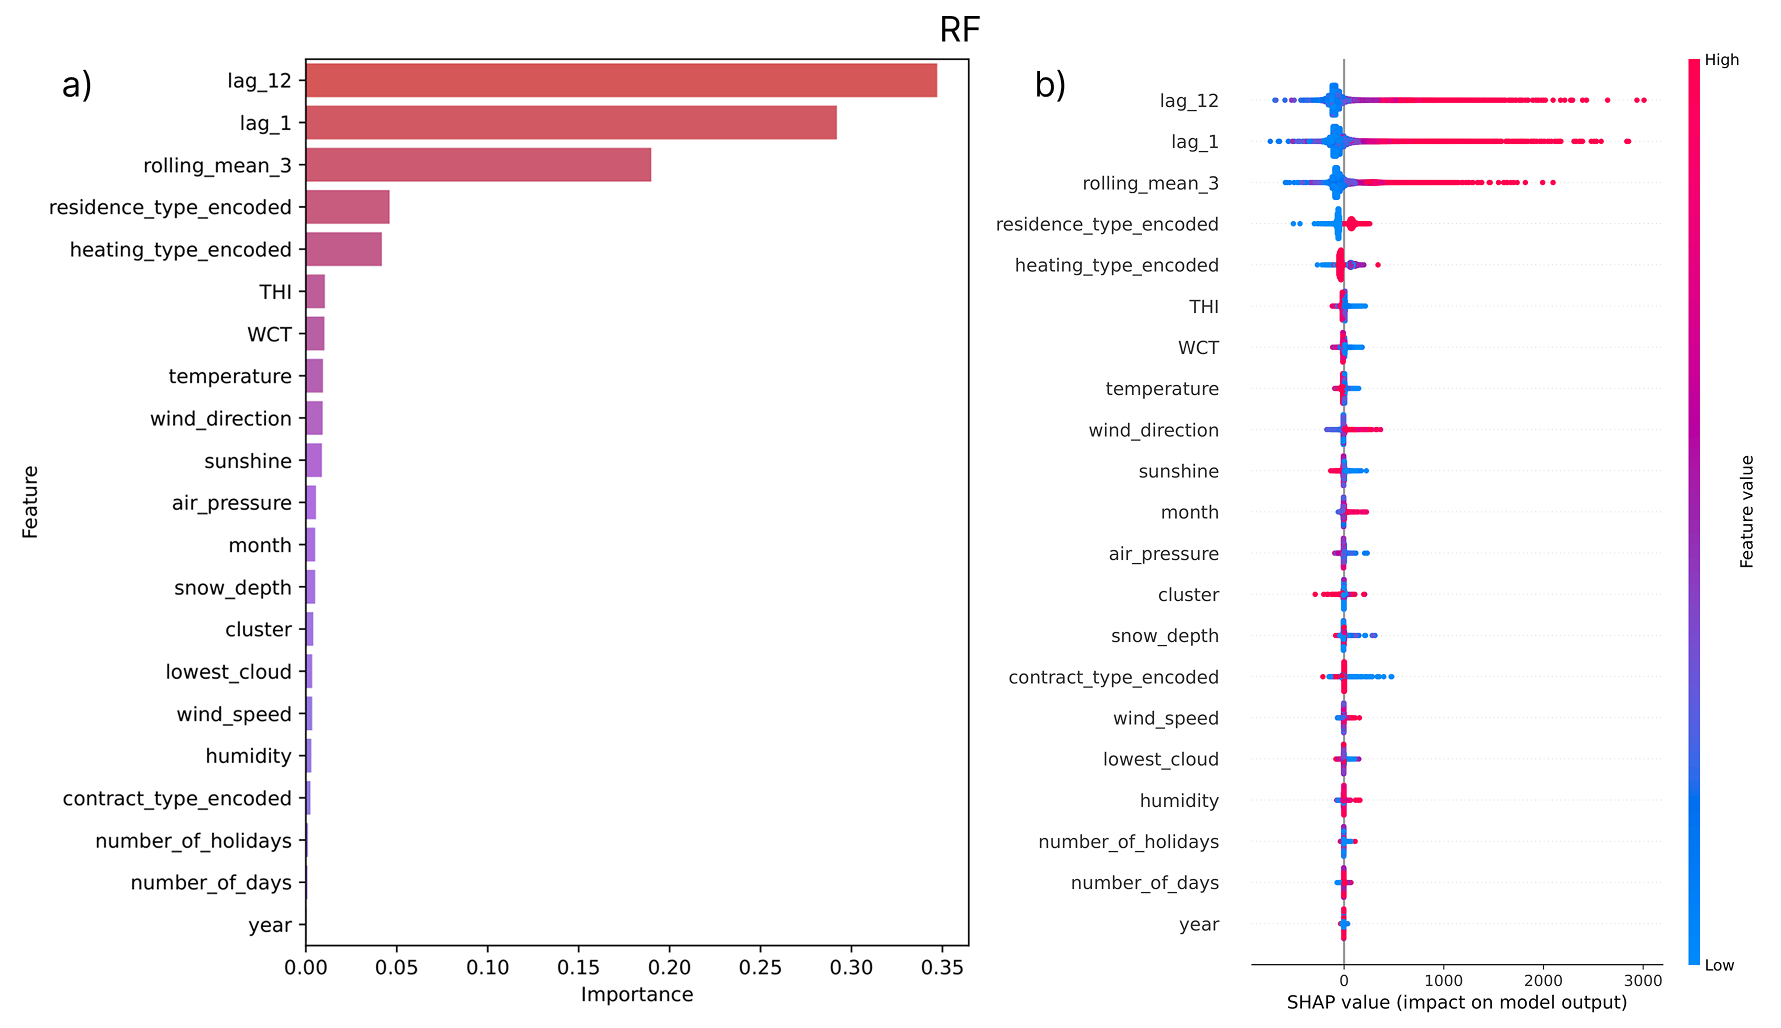
\includegraphics[width=1.25\linewidth]{figures/fi_shap_rf.png}
    }
    \caption{Feature importance and SHAP summary for RF.}
    \label{fig:fi-shap-rf}
\end{figure}

\begin{figure}[H]
    \centering
    \makebox[\linewidth][c]{%
        \hspace{-1.5cm}
        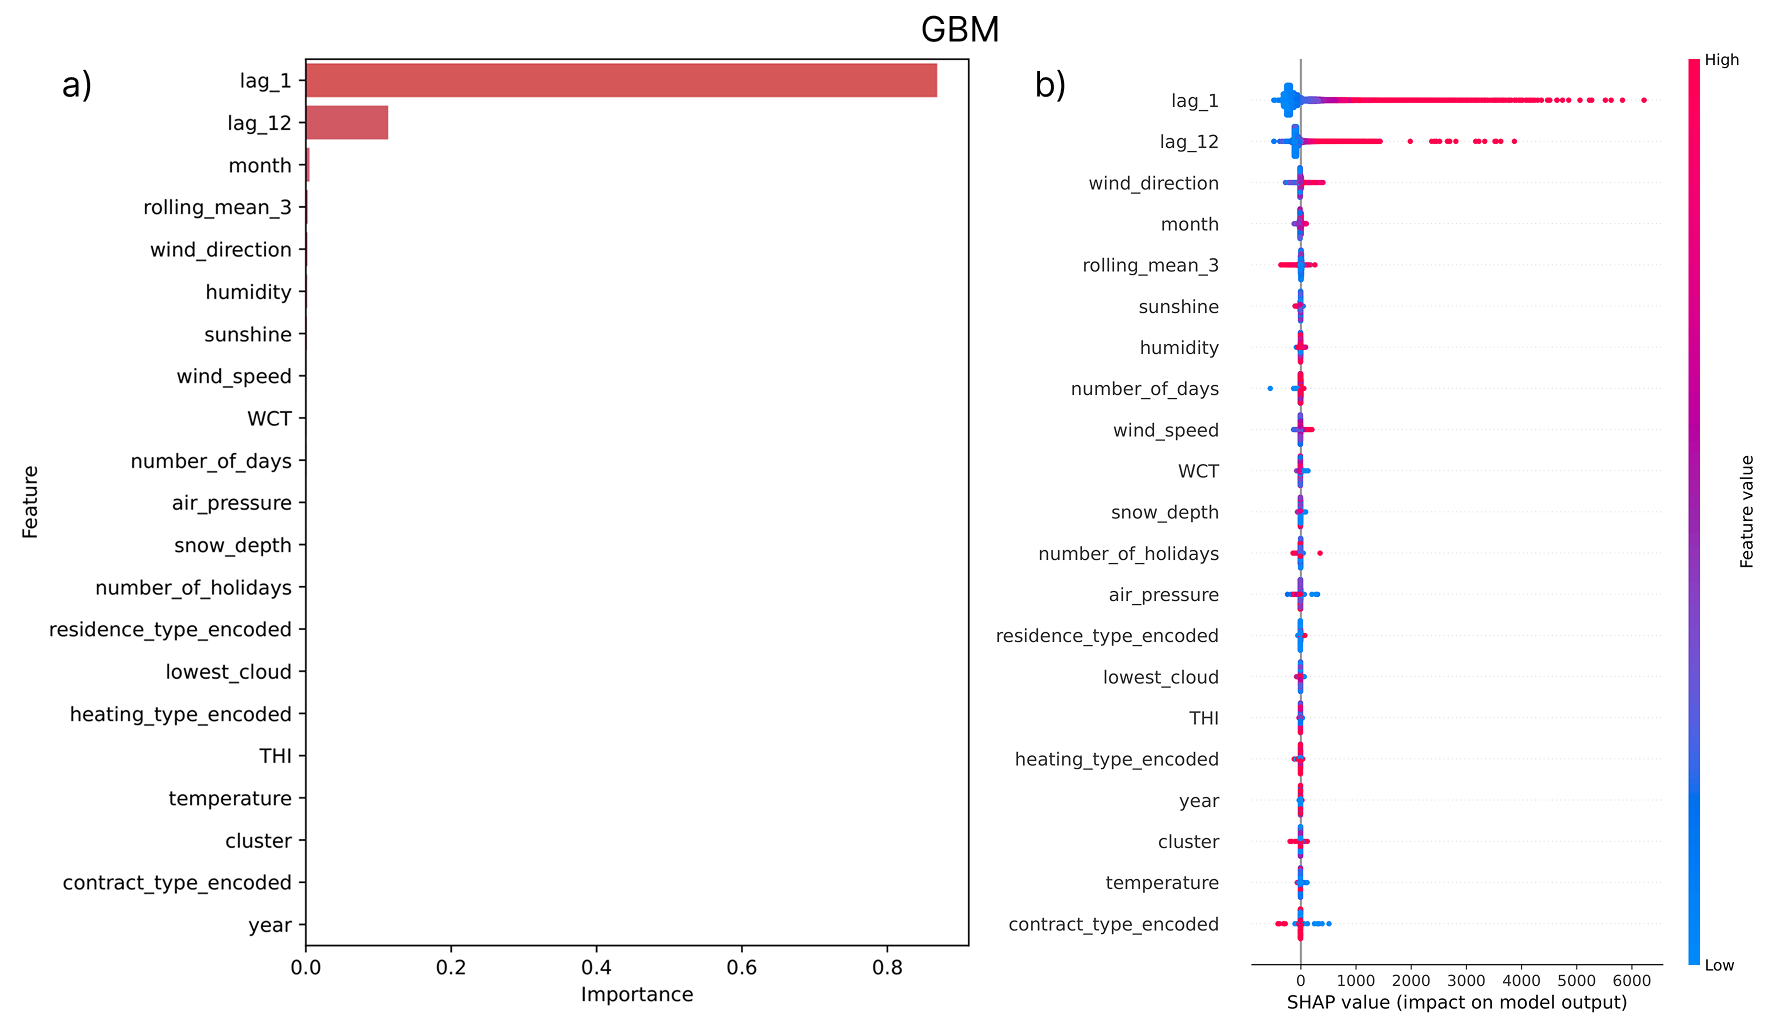
\includegraphics[width=1.25\linewidth]{figures/fi_shap_gbm.png}
    }
    \caption{Feature importance and SHAP summary for GBM.}
    \label{fig:fi-shap-gbm}
\end{figure}

\begin{figure}[H]
    \centering
    \makebox[\linewidth][c]{%
        \hspace{-1.5cm}
        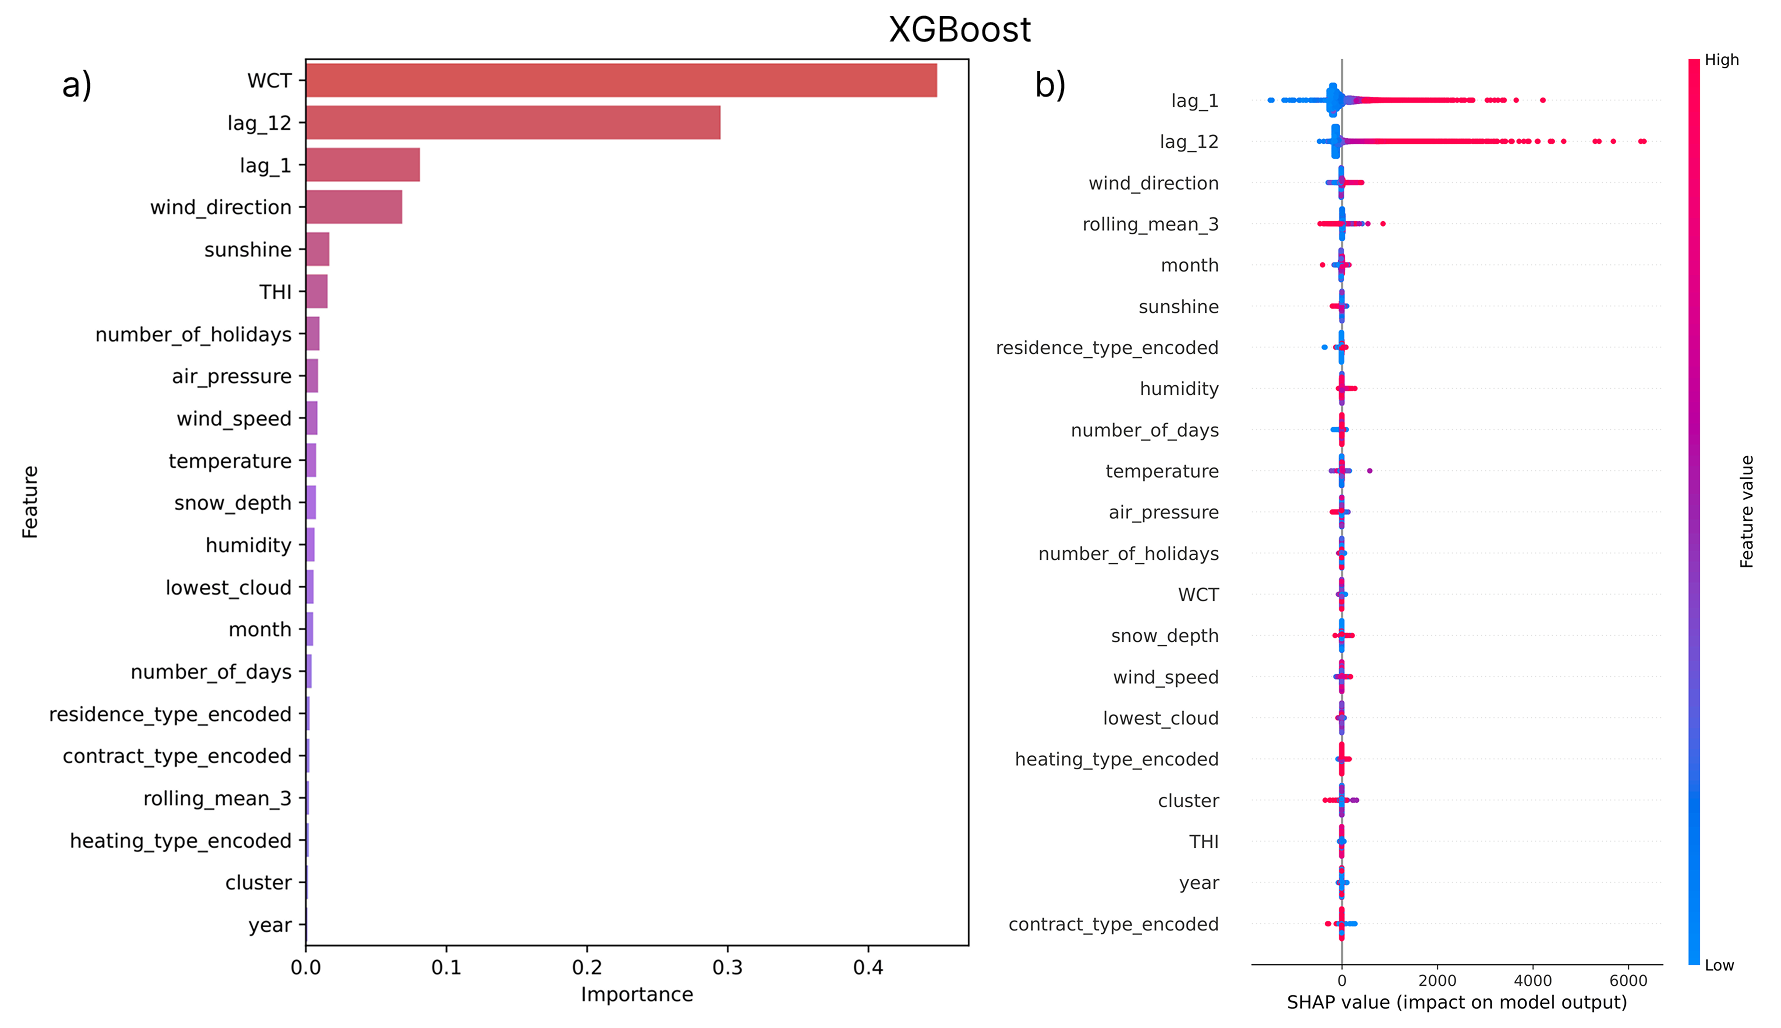
\includegraphics[width=1.25\linewidth]{figures/fi_shap_xgboost.png}
    }
    \caption{Feature importance and SHAP summary for XGBoost.}
    \label{fig:fi-shap-xgboost}
\end{figure}

\begin{figure}[H]
    \centering
    \makebox[\linewidth][c]{%
        \hspace{-1.5cm}
        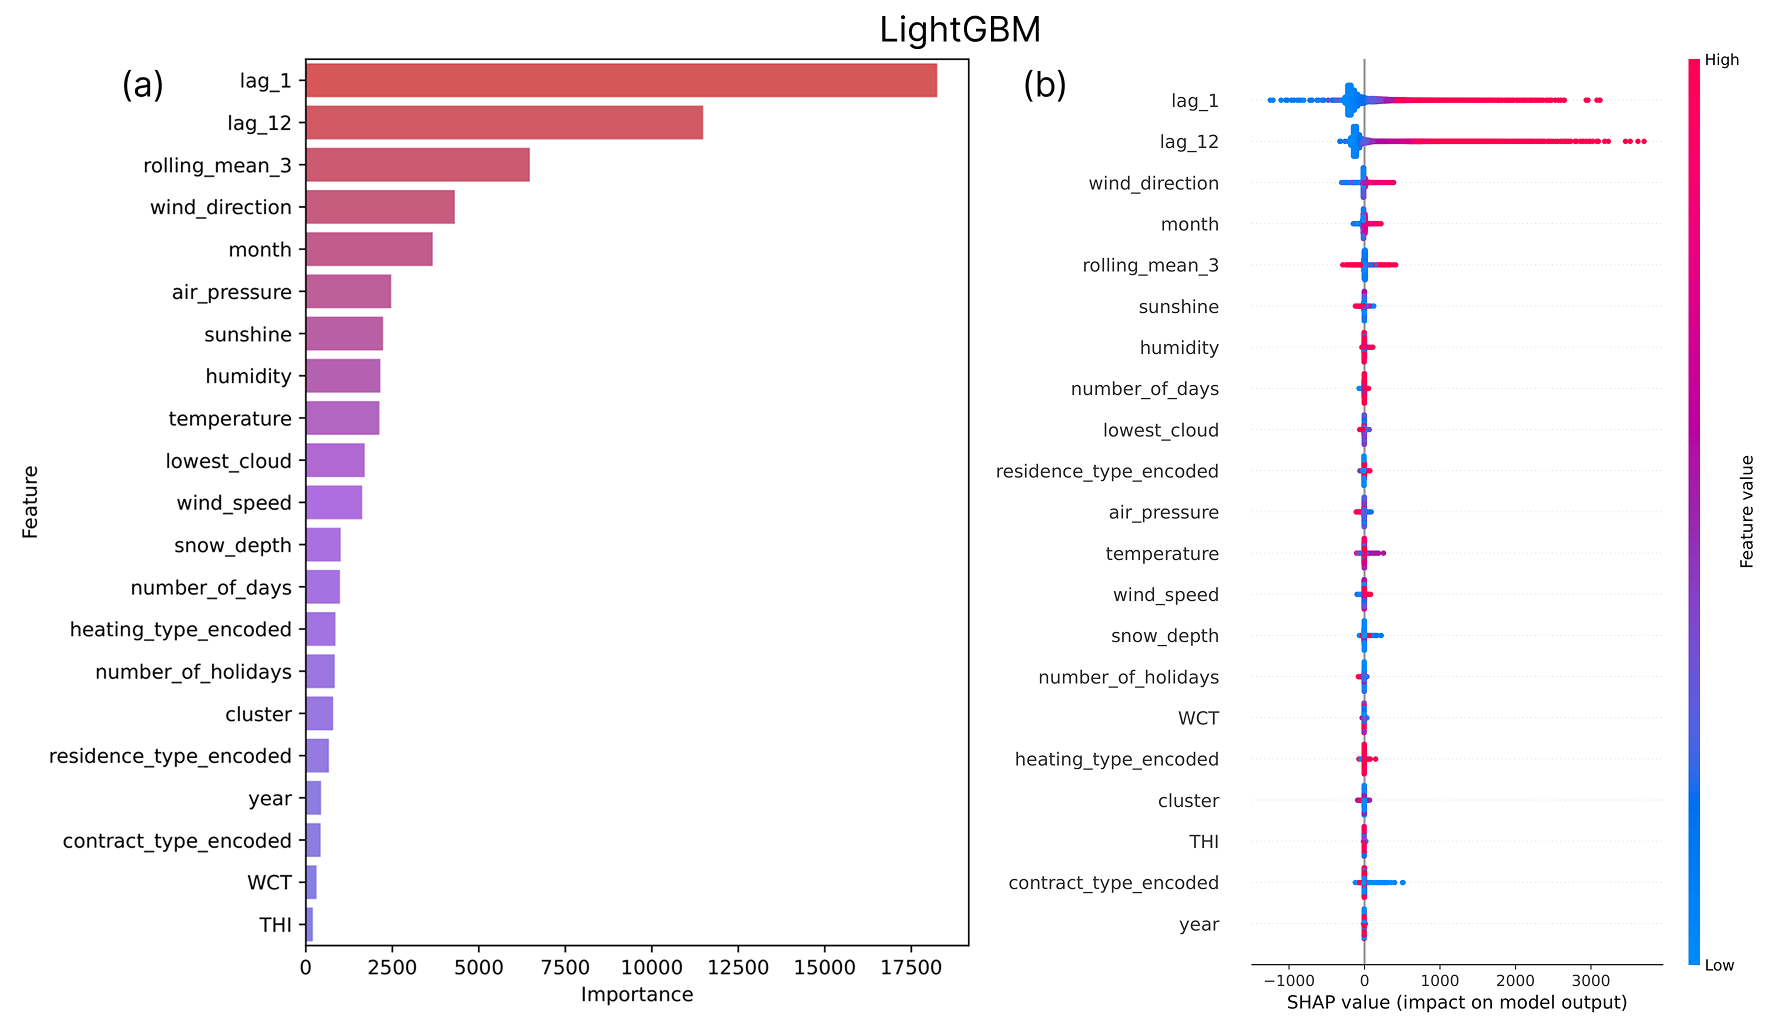
\includegraphics[width=1.25\linewidth]{figures/fi_shap_lgbm.png}
    }
    \caption{Feature importance and SHAP summary for LightGBM.}
    \label{fig:fi-shap-lgbm}
\end{figure}

\begin{figure}[H]
    \centering
    \makebox[\linewidth][c]{%
        \hspace{-1.5cm}
        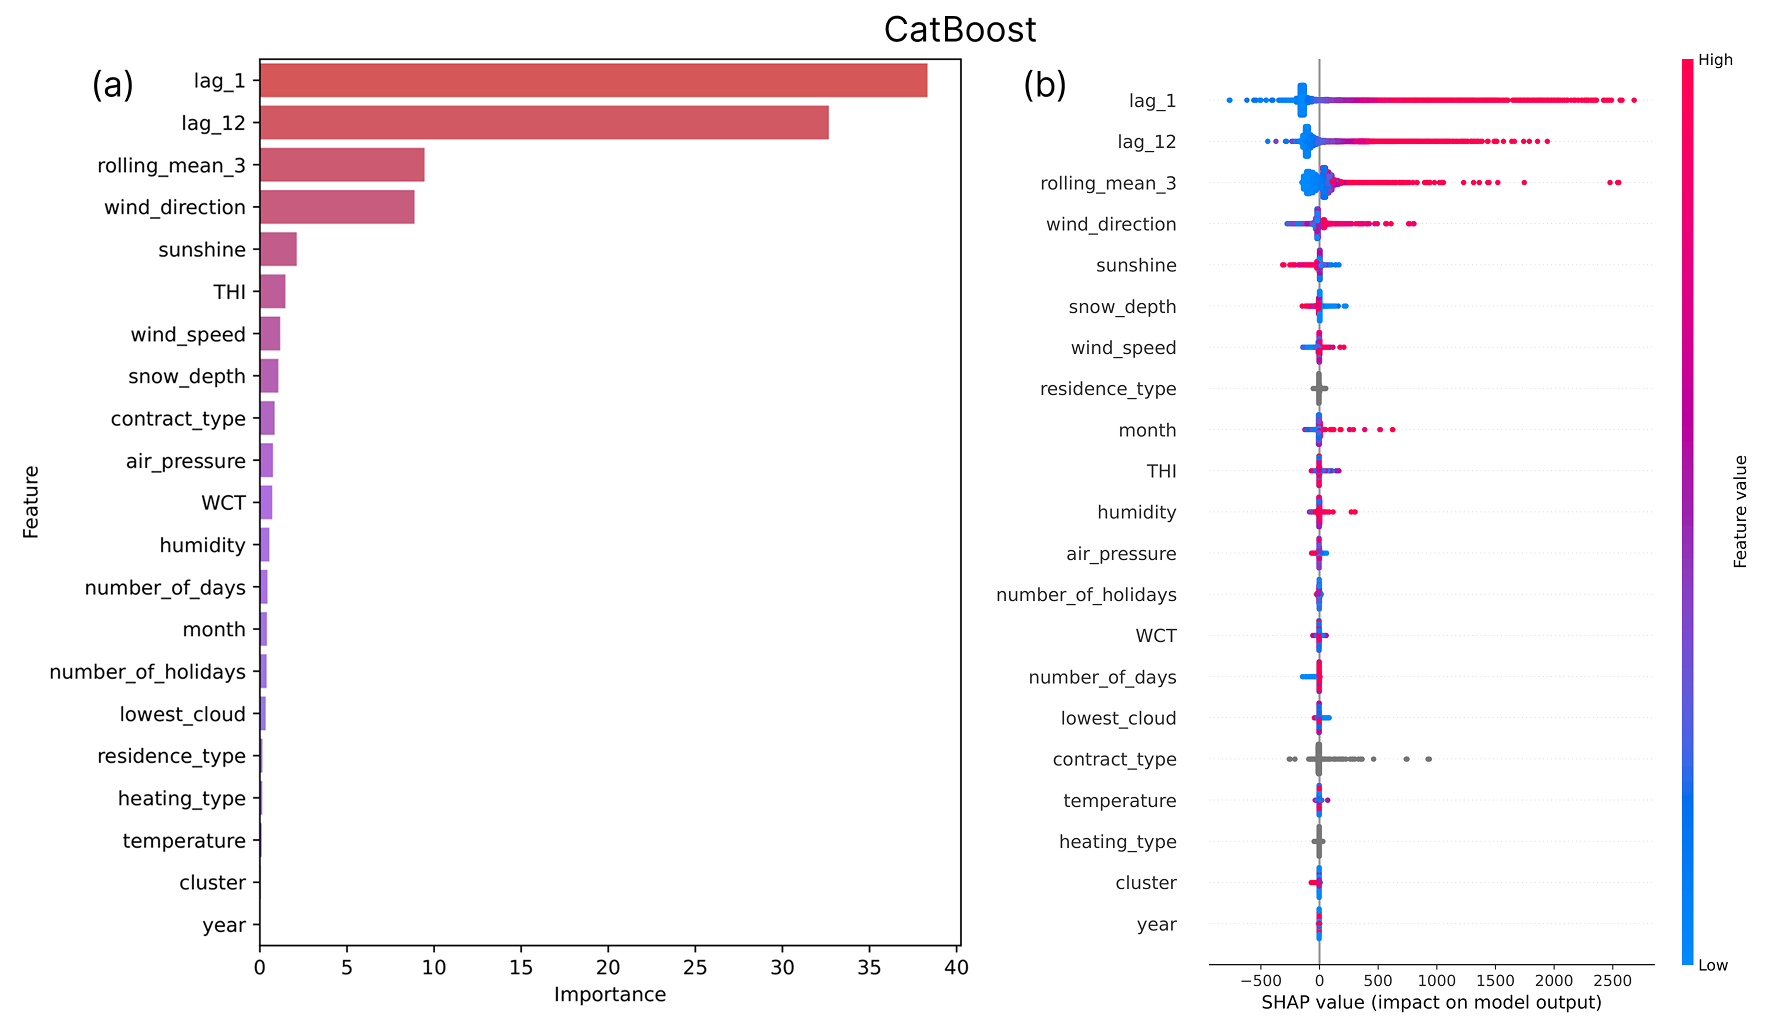
\includegraphics[width=1.25\linewidth]{figures/fi_shap_catboost.png}
    }
    \caption{Feature importance and SHAP summary for CatBoost.}
    \label{fig:fi-shap-catboost}
\end{figure}

\begin{comment}
\begin{figure}[H]
    \centering
    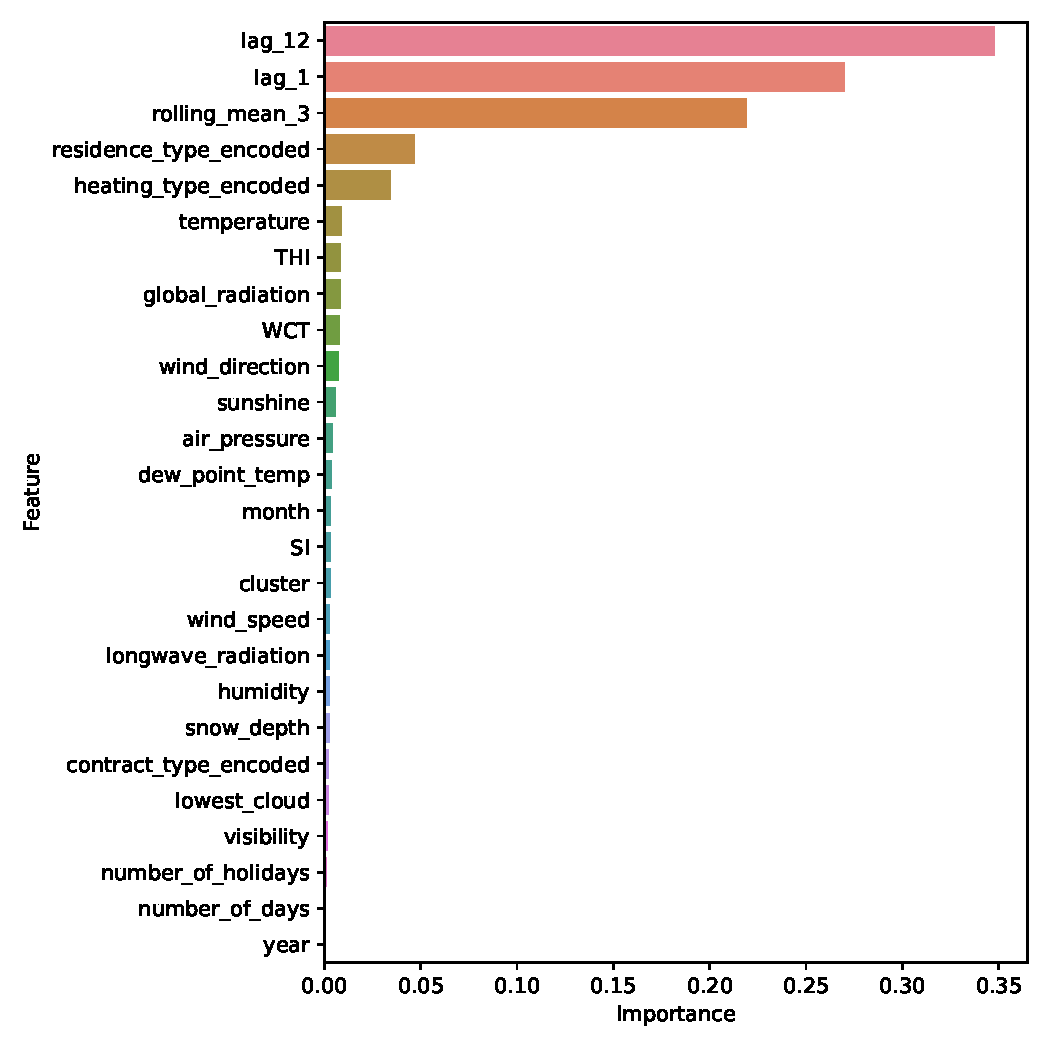
\includegraphics[width=0.9\linewidth]{figures/Fig4a_XAI_Feature_Importance_RF.pdf}
    \caption{Feature importances for RF.}
    \label{fig:feature-importances-rf}
\end{figure}

\begin{figure}[H]
    \centering
    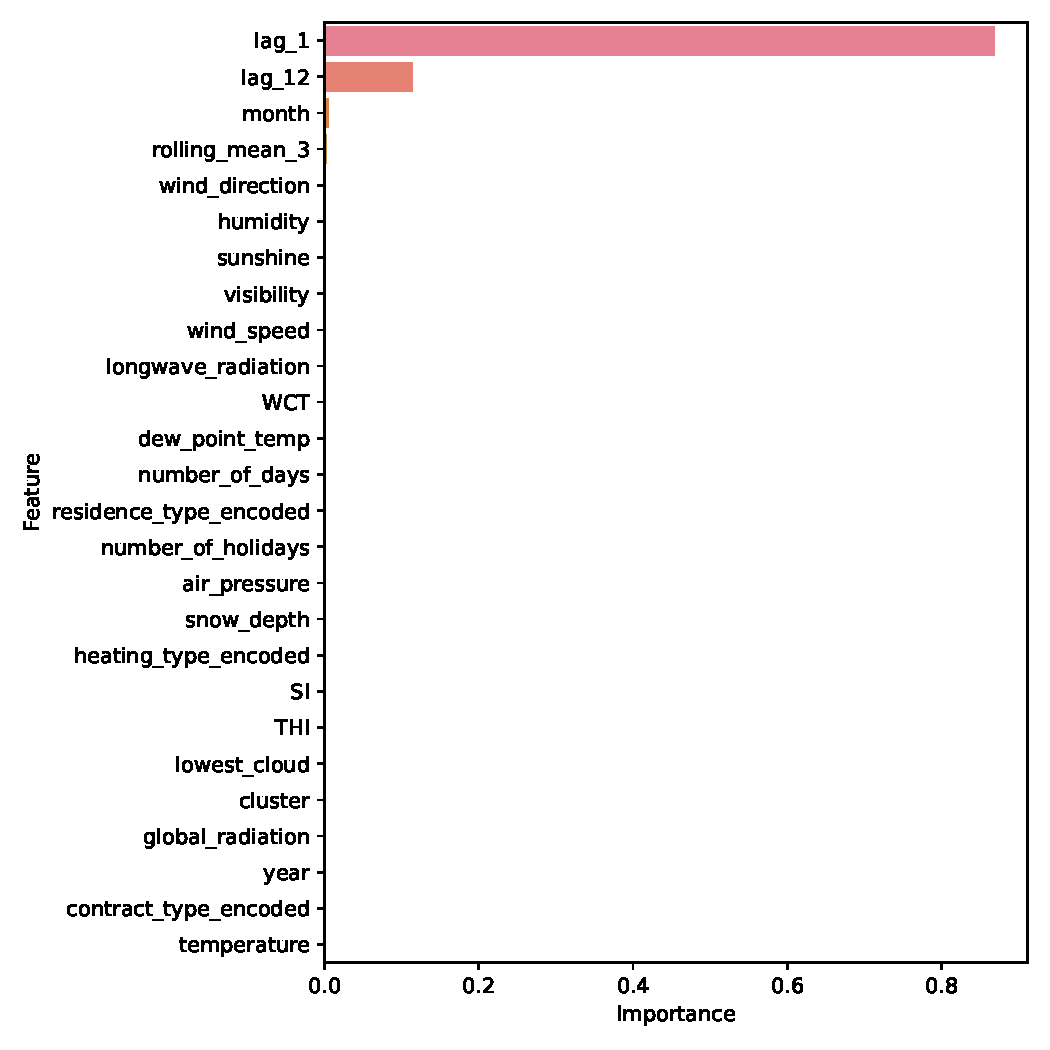
\includegraphics[width=0.9\linewidth]{figures/Fig4a_XAI_Feature_Importance_GBM.pdf}
    \caption{Feature importances for GBM.}
    \label{fig:feature-importances-gbm}
\end{figure}

\begin{figure}[H]
    \centering
    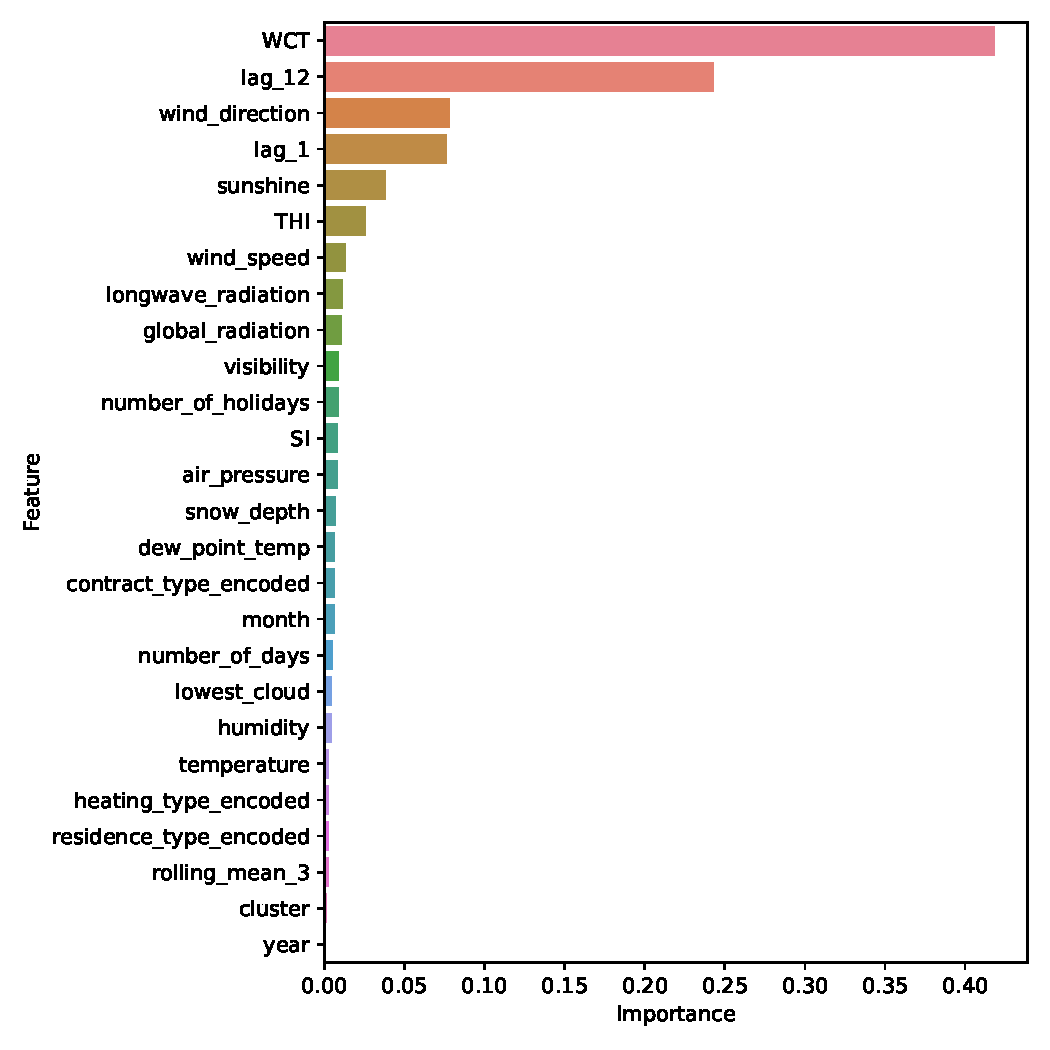
\includegraphics[width=0.9\linewidth]{figures/Fig4a_XAI_Feature_Importance_XGBoost.pdf}
    \caption{Feature importances for XGBoost.}
    \label{fig:feature-importances-xgboost}
\end{figure}

\begin{figure}[H]
    \centering
    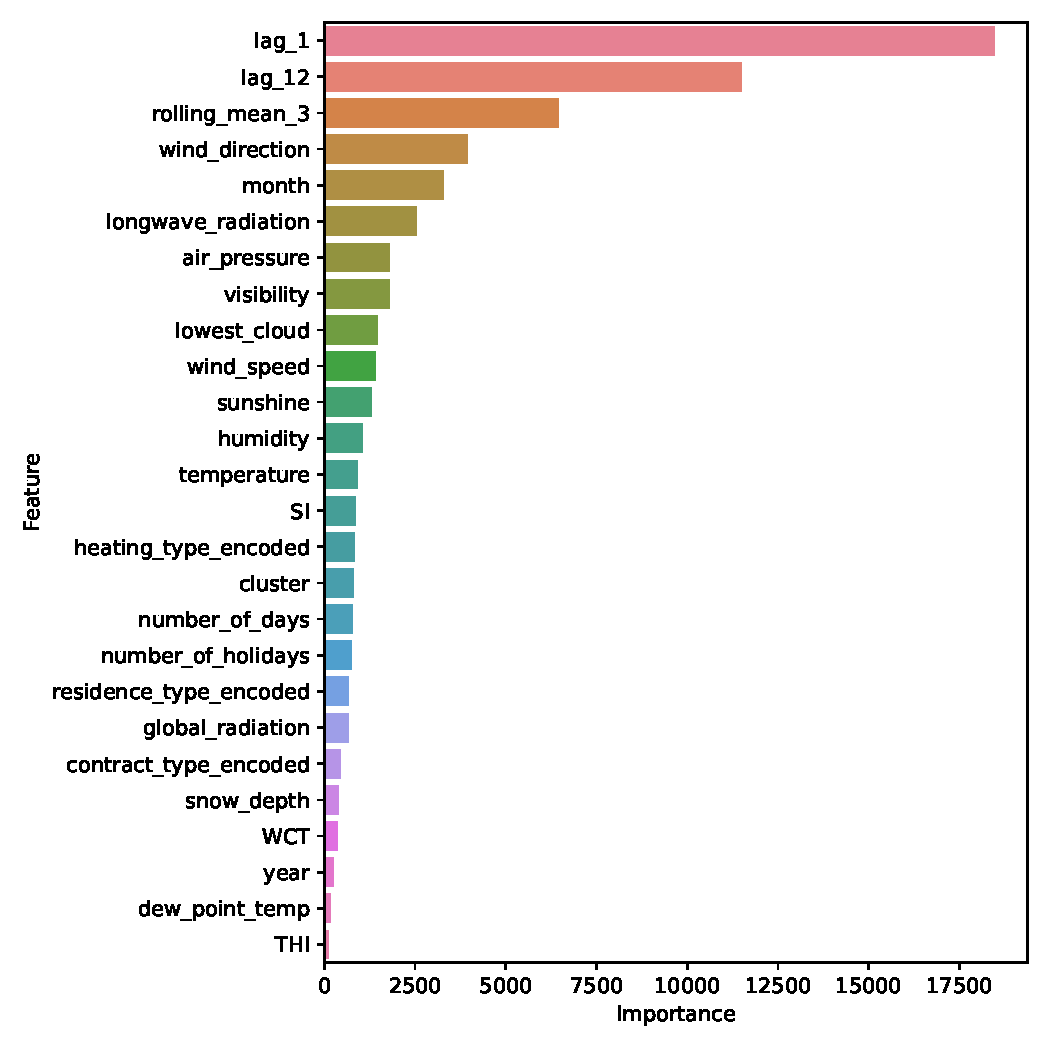
\includegraphics[width=0.9\linewidth]{figures/Fig4a_XAI_Feature_Importance_LightGBM.pdf}
    \caption{Feature importances for LightGBM.}
    \label{fig:feature-importances-lgbm}
\end{figure}

\begin{figure}[H]
    \centering
    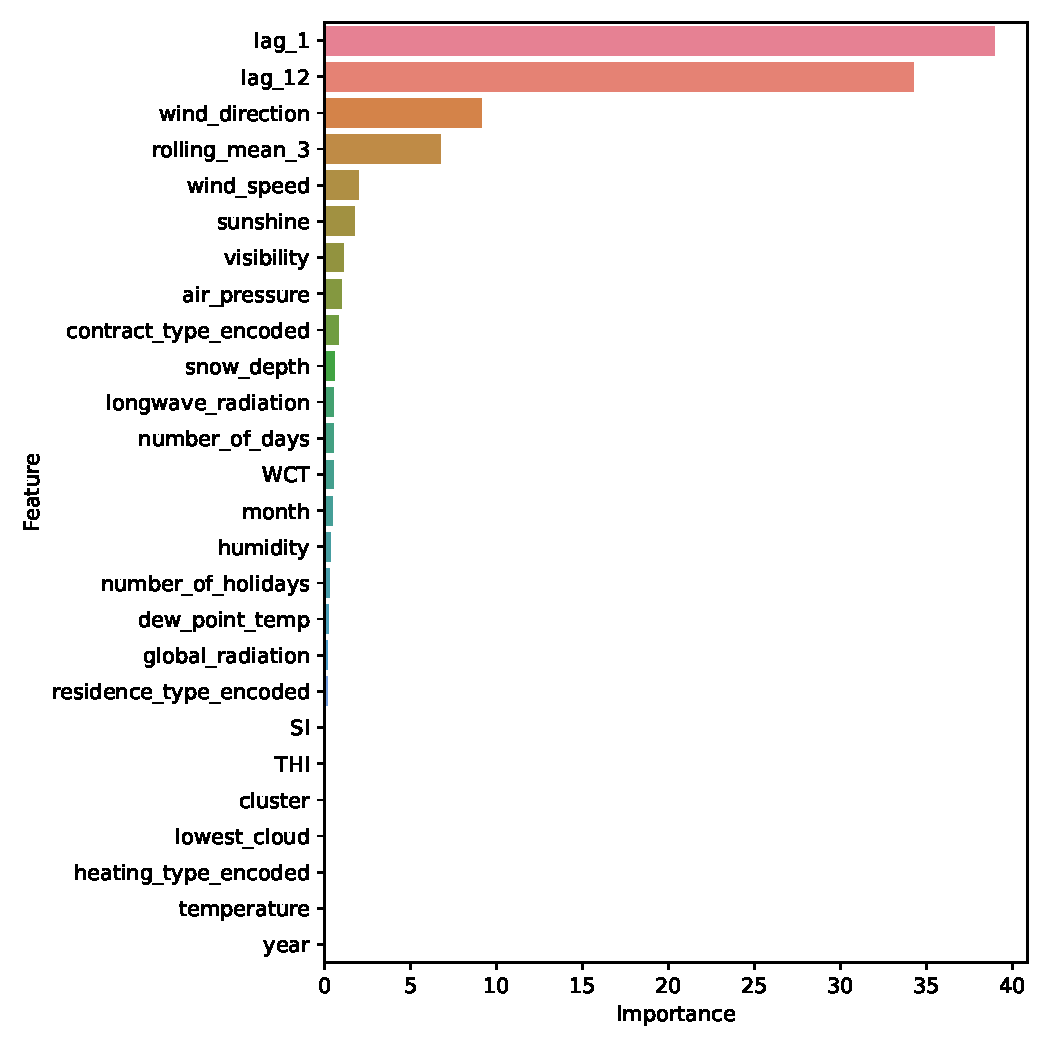
\includegraphics[width=0.9\linewidth]{figures/Fig4a_XAI_Feature_Importance_CatBoost.pdf}
    \caption{Feature importances for CatBoost.}
    \label{fig:feature-importances-catboost}
\end{figure}

\begin{figure}[H]
    \centering
    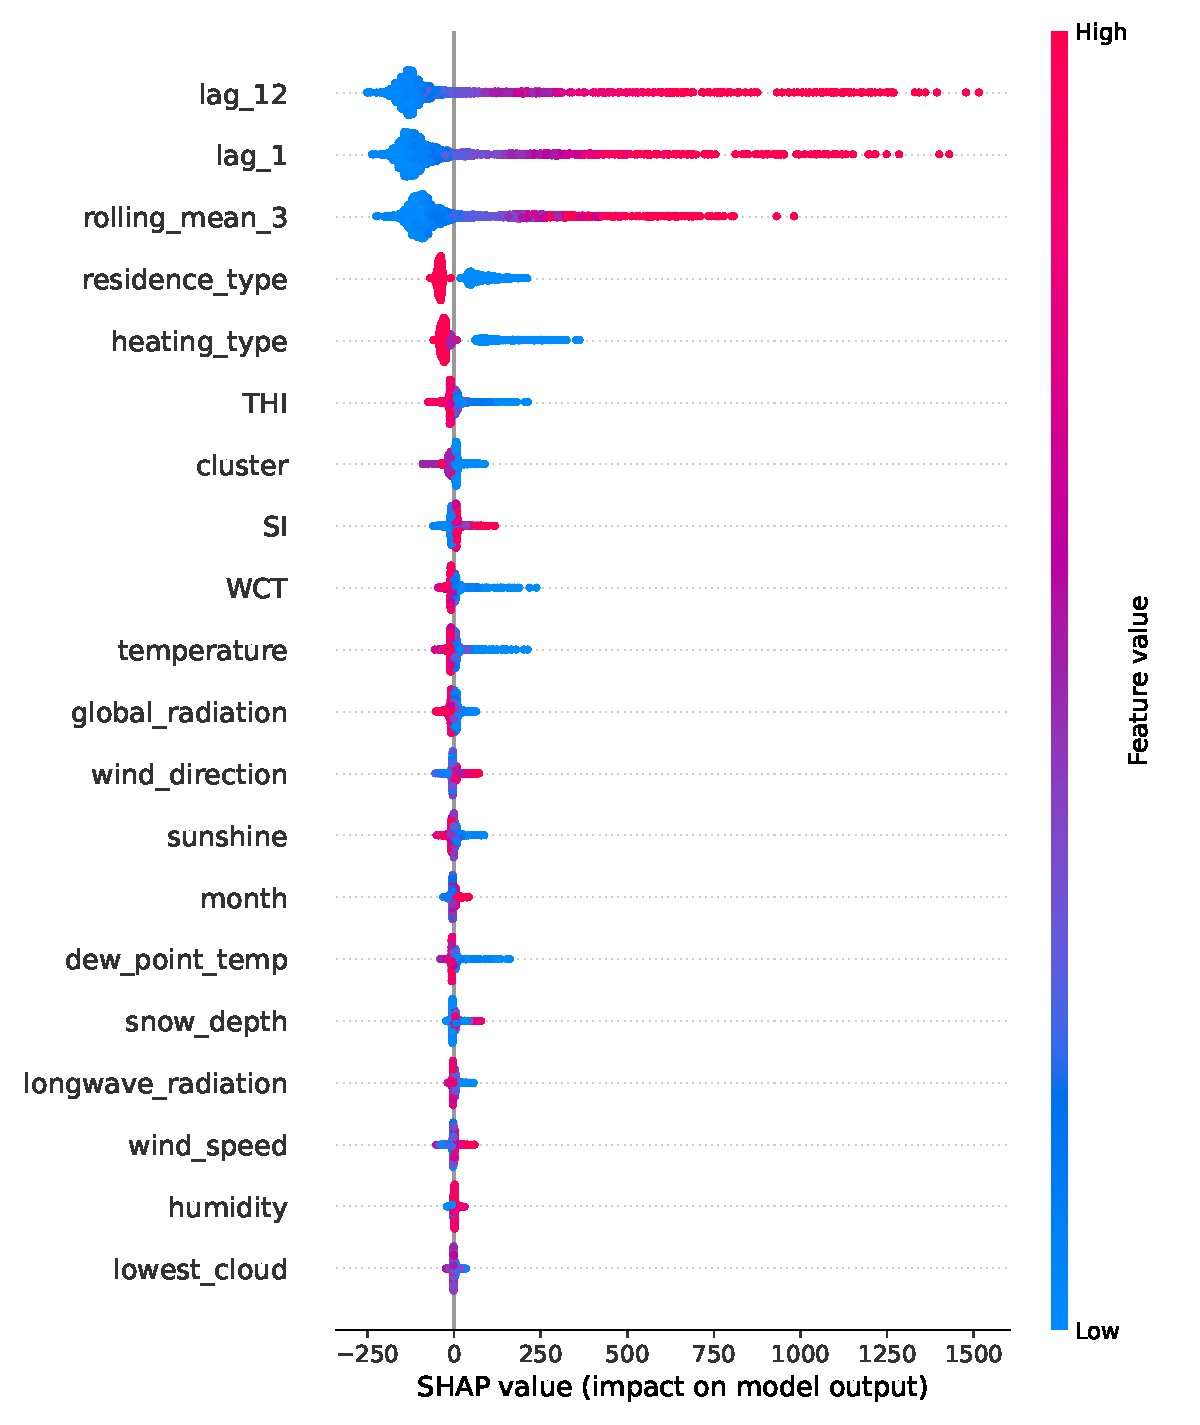
\includegraphics[width=0.9\linewidth]{figures/Fig4b_XAI_SHAP_Summary_RF.pdf}
    \caption{SHAP summary for RF [2000 sample with approximate shap values].}
    \label{fig:shap-summary-rf}
\end{figure}

\begin{figure}[H]
    \centering
    \includegraphics[width=0.9\linewidth]{figures/Fig4b_XAI_SHAP_Summary_GBM.pdf}
    \caption{SHAP summary for GBM [2000 sample].}
    \label{fig:shap-summary-gmb}
\end{figure}

\begin{figure}[H]
    \centering
    \includegraphics[width=0.9\linewidth]{figures/Fig4b_XAI_SHAP_Summary_XGBoost.pdf}
    \caption{SHAP summary for XGBoost [2000 sample].}
    \label{fig:shap-summary-xgboost}
\end{figure}

\begin{figure}[H]
    \centering
    \includegraphics[width=0.9\linewidth]{figures/Fig4b_XAI_SHAP_Summary_LightGBM.pdf}
    \caption{SHAP summary for Light GBM [2000 sample].}
    \label{fig:shap-summary-lgmb}
\end{figure}

\begin{figure}[H]
    \centering
    \includegraphics[width=0.9\linewidth]{figures/Fig4b_XAI_SHAP_Summary_CatBoost.pdf}
    \caption{SHAP summary for CatBoost [2000 sample].}
    \label{fig:shap-summary-catboost}
\end{figure}
\end{comment}